\bframe{Discrete}
\topline
\begin{equation*}
\dot{\mathbf{y}} = \mathbf{K}(t) \mathbf{y}
\end{equation*}

\begin{itemize}
\item Start with ortogonal vectors $\mathbf{y}^k$
\item Iterate
\item ``Gramm-Schmidt'' $\mathbf{y}^k$ and accumulate change
\end{itemize}
\eframe

\bframe{Discrete}
\topline
\begin{center}
  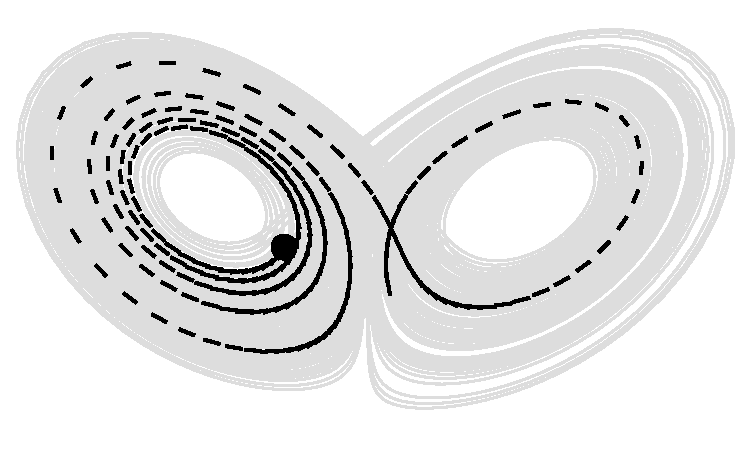
\includegraphics[width=\textwidth]{i/wolf.pdf}
\end{center}
\eframe

\bframe{Continues}
\topline

\begin{equation*}
\dot{\mathbf{y}} = \mathbf{K}(t) \mathbf{y}
\end{equation*}

\begin{equation*}
\dot{\mathbf{Y}} = \mathbf{K}(t) \mathbf{Y}
\end{equation*}

\begin{equation*}

\end{equation*}

\eframe
